\section{The Problem Setting}

\begin{frame}{The Problem Setting}
  \begin{figure}[htp]
      \includegraphics[width=12cm]{particles}
      \label{fig:particles}
  \end{figure}
  \vspace{9mm}
  $\boldsymbol{f}_{i}=\sum_{j=1, i \neq j}^{N} \boldsymbol{F}\left(\boldsymbol{x}_{i}-\boldsymbol{x}_{j}, q_{i} q_{j}\right)$\hspace{5cm}$\boldsymbol{F}(\Delta \boldsymbol{x}, Q)=-Q \frac{\Delta \boldsymbol{x}}{\|\Delta \boldsymbol{x}\|^{2}}$
\end{frame}

\section{A Single-Level Method}

\begin{frame}{2D Gravitational Potential}
  The FMM is defined in terms of the potential,
  \begin{equation}
    \Phi_y(\vct x) = \log(\vct x - \vct y) m_y
  \end{equation}
  where $\vct x$ and $\vct y$ are numbers in the complex plane (for the ease of notation).

  The force acting between two particles can be obtained from the potential:
  \begin{equation}
    f(\vct x) = -\nabla(\Re(\Phi)) = -\left(\Re\left(\der\Phi{\vct x}\right), -\Im\left(\der\Phi{\vct x}\right)\right)^T
  \end{equation}
\end{frame}

\begin{frame}{2D Gravitational Potential}
  \vfill
  \begin{figure}
    \centering
    \begin{tikzpicture}
      \begin{axis}[ width=0.5\textwidth
                  , xlabel={$\vct x - \vct y$}
                  , ylabel={$\Phi$}
                  , domain=-4:4
                  , samples=100
                  , xmin=-4, xmax= 4
                  , clip = false
                  ]
        \addplot+[very thick] {ln(abs(x))};
        \fill[Set1-D] (xticklabel* cs:0.5) circle (5pt);
      \end{axis}
    \end{tikzpicture}
  \end{figure}
  Note: smooth far away
\end{frame}

\begin{frame}{Outgoing Expansion}
  We wish to calculate the "felt potential" $\Psi$
  \begin{equation}
    \Psi(\vct x_i) = \sum_j^N \Phi(\vct x_i - \vct y_j)
  \end{equation}
  for many $\vct x_i$ ($i = 1 \dots M$) $\rightarrow \mathcal{O}(N\cdot M)$

  Idea: seperate contributions from positions $\vct x_i$ and $\vct y_j$,
  \begin{equation}
    \Psi(\vct x_i) \approx \sum_{p=0}^{P-1} B_p(\vct x_i) C_p(\vct y, m_{\vct y})
  \end{equation}
  with small constant $P$ $\rightarrow \mathcal{O}(N+M)$
\end{frame}

\begin{frame}{Outgoing Expansion}
  \begin{align}
    \Phi(\vct x) &= \log(\vct x - \vct y)
    = \log((\vct x - \vct c_\sigma) - (\vct y - \vct c_\sigma)) \\
    &= \log(\vct x - \vct c_\sigma) + \underbrace{\log \left(1 - \frac{\vct y - \vct c_\sigma}{\vct x - \vct c_\sigma} \right)}%
      _\text{Taylor expansion around $\frac{\vct y - \vct c_\sigma}{\vct x - \vct c_\sigma} = 0$} \\
    &= \log(\vct x - \vct c_\sigma) - \sum_{k=1}^\infty \frac 1k \frac{(\vct y - \vct c_\sigma)^k}{(\vct x - \vct c_\sigma)^k}
  \end{align}
\end{frame}

\begin{frame}{Outgoing Expansion}
  \begin{equation}
    \Phi(\vct x) = \log(\vct x - \vct c_\sigma) - \sum_{k=1}^\infty \frac 1k \frac{(\vct y - \vct c_\sigma)^k}{(\vct x - \vct c_\sigma)^k}
  \end{equation}

  \begin{equation}
    \Psi(\vct x_i) = \sum_j^N \Phi(\vct x_i - \vct y_j) m_j
    = q_0 \log(\vct x - \vct c_\sigma) + \sum_{k=1}^\infty \frac{q_k}{(\vct x - \vct c_\sigma)^k}
  \end{equation}

  \begin{block}{Outgoing Expansion}
    \begin{equation}
      \begin{split}
        q_0 &= \sum_j^N m_j \\
        q_k &= - \sum_j^N \frac{m_j}{k} (\vct y - \vct c_\sigma)^k
      \end{split}
    \end{equation}
  \end{block}
\end{frame}

\begin{frame}{Outgoing Expansion}
  \vfill
  \begin{figure}
    \centering
    \begin{tikzpicture}
      \begin{axis}[ width=0.5\textwidth
                  , xlabel={$\vct x - \vct c_\sigma$}
                  , ylabel={$\Phi$}
                  , samples=100
                  , xmin=-1, xmax= 4
                  , ymin=-8, ymax= 4
                  , clip = false
                  , legend pos = outer north east
                  ]
        \addplot+[very thick, domain=-0.999:4] {ln(x+0.9) + ln(x+0.7)};
        \addlegendentry{Exact potential}

        \fill[Set1-D] (xticklabel* cs:0.02) circle (5pt);
        \fill[Set1-D] (xticklabel* cs:0.06) circle (5pt);
        \fill[Set1-E] (xticklabel* cs:0.2) circle (5pt);

        \addplot+[very thick, domain=0.03:4] {2*ln(x)};
        \addplot+[very thick, domain=0.4:4] {2*ln(x) -(-0.9-0.7)/x -1/2*(0.9^2+0.7^2)/x^2 -1/3*(-0.9^3-0.7^3)/x^3};
        \addlegendentry{Expansion $P=1$}
        \addlegendentry{Expansion $P=4$}
      \end{axis}
    \end{tikzpicture}
  \end{figure}
\end{frame}

\begin{frame}{Incoming Expansion}
  \vfill
  The outgoing expansion is an efficient way to calculate forces between to seperated clusters of particles.

  \onslide<2>{Idea: Divide domain into equisized boxes and use outgoing expansion to compute long-distance potentials.}

  \vfill
  \begin{figure}
    \centering
    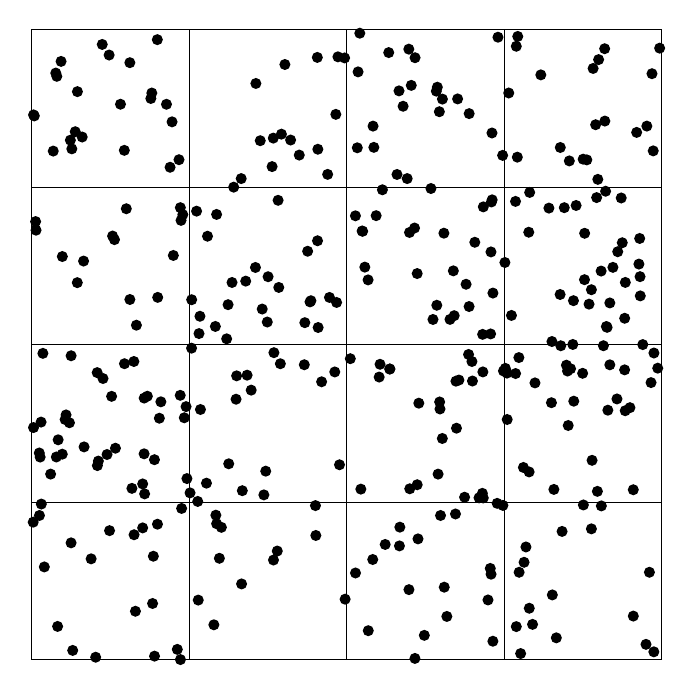
\begin{tikzpicture}
      \draw (0,0) rectangle (8,8);
      \onslide<1>{
        \foreach \x in {1,...,20} {
          \fill (2*rnd  , 2*rnd+2) circle (2pt);
          \fill (2*rnd+6, 2*rnd+3) circle (2pt);
        }
      }
      \onslide<2>{
        \draw[step=2] (0,0) grid (8,8);
        \foreach \x in {1,...,320} {
          \fill (rnd*8, rnd*8) circle (2pt);
        }
      }
    \end{tikzpicture}
  \end{figure}
\end{frame}

\begin{frame}{Incoming Expansion}
  \begin{equation}
    \Psi(\vct x_i)
    \approx \underbrace{\sum_{j=1}^n \Psi_j(\vct x_i)}_\text{outgoing expansions (long-distance)}
    + \underbrace{\sum_{j=1}^m \Phi(\vct x_i - \vct y_j)}_\text{direct interactions (short-distance)}
  \end{equation}

  Problem: We need to calculate interactions with \emph{all} outgoing expansions for \emph{every} particle $\rightarrow \mathcal{O}(M\cdot n)$;

  Idea: Find approximation $\sum_{j=1}^n \Psi_j(\vct x_i) \approx \Psi(\vct x_i) \rightarrow \mathcal{O}(M+n)$
\end{frame}

\begin{frame}{Incoming Expansion}
  \begin{align}
    \Psi(\vct x_i) &= \sum_{j=1}^n \Psi_j(\vct x_i) \\
    &= \sum_{j=1}^n \left( q_0 \log(\vct x - \vct c_\sigma) + \sum_{k=1}^\infty \frac{q_k}{(\vct x - \vct c_\sigma)^k} \right) \\
    &= \sum_{j=1}^n \left( q_0 \log((\vct x -\vct c_\tau) - (\vct c_\sigma - \vct c_\tau)) + \sum_{k=1}^\infty \frac{q_k}{((\vct x -\vct c_\tau) - (\vct c_\sigma - \vct c_\tau))^k} \right) \\
    &= \dots \\
    &= \sum_{j=1}^n \sum_{k=0}^\infty v_{j,k} (\vct x_i - \vct c_\tau)^k \\
    &= \sum_{k=0}^\infty (\vct x_i - \vct c_\tau)^k \sum_{j=1}^n v_{j,k}
  \end{align}
\end{frame}

\begin{frame}{Incoming Expansion}
  \begin{block}{Incoming Expansion}
    \begin{equation}
      \begin{split}
        v_0 &= q_0 \log(\vct c_\tau - \vct c_\sigma) + \sum_{j=1}^\infty q_j (-1)^j \frac 1 {(\vct c_\sigma - \vct c_\tau)^j} \\
        v_k &= -q_0 \frac 1 {k(\vct c_\sigma - \vct c_\tau)^k} + \sum_{j=1}^\infty q_j (-1)^j \mat{k+j-1\\j-1} \frac 1 {(\vct c_\sigma - \vct c_\tau)^{k+j}} \\
      \end{split}
    \end{equation}
  \end{block}
\end{frame}

\begin{frame}{Incoming Expansion}
  \vfill
  \begin{figure}
    \centering
    \begin{tikzpicture}
      \begin{axis}[ width=0.5\textwidth
                  , xlabel={$\vct x - \vct c_\tau$}
                  , ylabel={$\Phi$}
                  , samples=100
                  , domain=-2.5:2.5
                  , xmin=-2.5, xmax= 2.5
                  , ymin=-8, ymax= 4
                  , clip = false
                  , legend pos = outer north east
                  ]
        \addplot+[very thick] {ln(abs(x+1.9)) + ln(abs(x+1.7)) + ln(abs(x-2.4)) + ln(abs(x-2.1))};
        \addlegendentry{Exact potential}

        \fill[Set1-D] (xticklabel* cs:0.12) circle (5pt);
        \fill[Set1-D] (xticklabel* cs:0.16) circle (5pt);
        \fill[Set1-D] (xticklabel* cs:0.98) circle (5pt);
        \fill[Set1-D] (xticklabel* cs:0.92) circle (5pt);
        \fill[Set1-E] (xticklabel* cs:0.1) circle (5pt);
        \fill[Set1-E] (xticklabel* cs:0.9) circle (5pt);
        \fill[Set1-G] (xticklabel* cs:0.5) circle (5pt);

        \addplot+[very thick, domain=-1.9:1.9] {2*ln(abs(x+2)) -(0.1+0.3)/(x+2) + 2*ln(abs(x-2)) -(0.4+0.1)/(x-2)};
        \addplot+[very thick, domain=-1.9:1.9] {2*ln(abs(x+2))+2*ln(abs(x-2)) +0.4/(-2) +0.5/2 + (0.4/4 +0.5/4)*x};
        \addlegendentry{Outgoing expansions $P=2$}
        \addlegendentry{Incoming expansion $P=2$}
      \end{axis}
    \end{tikzpicture}
  \end{figure}
\end{frame}

\begin{frame}{TODO}
  $\mathcal O(n^{\nicefrac 43})$
\end{frame}
